\def\pgfsysdriver{pgfsys-dvipdfm.def}
%\documentclass[aspectratio=1610]{beamer}
\documentclass{beamer}
\usetheme[progressbar=head, titleformat=allcaps,block=fill]{metropolis}
\usepackage[orientation=landscape,size=custom,width=16,height=11.15,scale=.5,debug]{beamerposter}

%%% PACKAGES AND INPUTS
\usepackage{pgfopts}
\usepackage{pgfpages}
\usepackage{graphicx}
\usepackage{xcolor}
\usepackage{tikz}
\usetikzlibrary{3d,hyperref}
\usepackage{verbatim}
\usepackage{comment}
%\input{153controls}
\usepackage{pgfplots}
\usepackage{linalgjh}

\usepackage{multicol}


%%% POLAR SETUP
\usepgfplotslibrary{polar}
\pgfplotsset{compat=1.10}
\pgfplotsset{mypolarplot/.style={%
  clip=false, % needed for double line (last \addplot command)
  domain=0:360, % plot full cycle
  samples=180, % number of samples; can be locally adjusted
  grid=both, % display major and minor grids
  major grid style={black}, 
  minor x tick num=3, % 3 minor x ticks between majors
  minor y tick num=1, % 1 minor y tick between majors
  xtick={0,45,...,359},
  xticklabels={%
    $0$,
    $\frac{ \pi}{4}$,
    $\frac{ \pi}{2}$,
    $\frac{3\pi}{4}$,
    $\pi$,
    $\frac{5\pi}{4}$,
    $\frac{3\pi}{2}$,
    $\frac{7\pi}{4}$
  },
  yticklabel style={anchor=north}, % move label position
}}

%%%% COLORS
\definecolor{gold}{HTML}{ffb81c}
\definecolor{heypurple}{HTML}{6B0FFF}
\definecolor{darkgold}{HTML}{5A440D}
\definecolor{darkblue}{HTML}{00268D}
\definecolor{proof}{RGB}{55,54,172}
\definecolor{nicegreen}{RGB}{0,127,35}
\definecolor{remgrey}{RGB}{179,179,179}
\definecolor{Purple}{HTML}{3C0940}
\definecolor{darkgreen}{HTML}{214009}
\definecolor{Orange}{HTML}{7F2000}
\definecolor{Blue}{HTML}{003E78}
\definecolor{Gold}{HTML}{FFCB0A}
\definecolor{gvsublue1}{HTML}{0065a4}
\definecolor{gvsublue2}{HTML}{88B3DA}
\definecolor{unlred}{HTML}{D00000}
\definecolor{DordtGrey}{RGB}{127,127,127}
\definecolor{newred}{HTML}{85140D}
\definecolor{msugreen}{HTML}{023328}
\definecolor{seafoam}{HTML}{127F67}
\definecolor{mnmaroon}{HTML}{790018}
\definecolor{mngold}{HTML}{FFD75F}
\definecolor{fallfoliage}{HTML}{763626}
\definecolor{stone}{HTML}{336B87}
\definecolor{shadow}{HTML}{2A3132}
\definecolor{grass}{HTML}{486B00}
\definecolor{thundercloud}{HTML}{505160}
\definecolor{meadow}{HTML}{598234}
\definecolor{ink}{HTML}{20232A}
\definecolor{rubyred}{HTML}{A01D26}
\definecolor{stormysea}{HTML}{335252}
\definecolor{rust}{HTML}{AA4B41}
\definecolor{forest}{HTML}{1E434C}
\definecolor{crimson}{HTML}{8D230F}
\definecolor{vtgold}{HTML}{C99E10}
\definecolor{vtrust}{HTML}{9B4F0F}

%%%% BEAMER THEMES AND OPTIONS
%\usetheme[progressbar=head,block=fill]{metropolis}
%\setbeameroption{show notes on second screen}
%\metroset{titleformat=smallcaps,block=transparent}
%\usecolortheme{owl}
\setbeamercolor{progress bar}{fg=heypurple,bg=heypurple!30}
\setsansfont[BoldFont={Graphik Semibold},Numbers={Produkt}]{Graphik}


%%% Dordt
%\setbeamercolor{alerted text}{fg=gold}
%\setbeamercolor{normal text}{fg=black}
%%%\setbeamercolor{block}{transparent}
%%%\setbeamercolor{sectionpage}{bg=white}
%%%\setbeamercolor{titleformatpage}{bg=white}
%\setbeamercolor{frametitle}{fg=gold,bg=black!2}
%%%%% GREEN OPTION
%%%\setbeamercolor{alerted text}{fg=seafoam} 
%%%\setbeamercolor{frametitle}{bg=msugreen}



%%% Purple
\setbeamercolor{alerted text}{fg=heypurple}
\setbeamercolor{normal text}{fg=black}
%%\setbeamercolor{block}{transparent}
%%\setbeamercolor{sectionpage}{bg=white}
%%\setbeamercolor{titleformatpage}{bg=white}
\setbeamercolor{frametitle}{fg=heypurple,bg=black!2}
%%%% GREEN OPTION
%%\setbeamercolor{alerted text}{fg=seafoam} 
%%\setbeamercolor{frametitle}{bg=msugreen}

%%% MN OPTION
%\setbeamercolor{alerted text}{fg=gold}
%\setbeamercolor{frametitle}{bg=mnmaroon}

%%% FALL MOUNTAIN
%\setbeamercolor{alerted text}{fg=fallfoliage}
%\setbeamercolor{frametitle}{bg=shadow}
%\setbeamercolor{alerted text}{fg=stone}
%\setbeamercolor{alerted text}{fg=grass}

%%% ICELAND
%\setbeamercolor{alerted text}{fg=meadow}
%\setbeamercolor{frametitle}{bg=thundercloud}


%%% VERMONT
%\setbeamercolor{alerted text}{fg=crimson}
%\setbeamercolor{alerted text}{fg=vtrust}
%\setbeamercolor{frametitle}{bg=thundercloud}


%%% INDUSTRIAL
%\setbeamercolor{alerted text}{fg=rubyred}
%\setbeamercolor{frametitle}{bg=ink}

%%% SAN FRANCISCO
%\setbeamercolor{alerted text}{fg=rust}
%\setbeamercolor{frametitle}{bg=stormysea}


%%%% MACROS
\def\rem#1{{\hfill \textit{\tiny {\color{remgrey} {#1}}}}}
\def\h#1{\alert{#1}}
\def\C{{\mathbb C}}
\def\Z{{\mathbb Z}}
\def\F{{\mathbb F}}
\def\bF{{\mathbb F}}
\def\Q{{\mathbb Q}}
\def\R{{\mathbb R}}
\def\P{{\mathbb P}}
\def\A{{\mathbb A}}
\def\N{{\mathbb N}}
\def\i{\mathbf i}}
\def\j{\mathbf j}}
\def\k{\mathbf k}}
\def\proj{{\text{proj}}}
\def\comp{{\text{comp}}}
\def\set#1{\left\{ {#1} \right\}}
\def\setof#1#2{{\left\{#1\,:\,#2\right\}}}


%%%% ENVIRONMENTS
\newenvironment{proof-idea}{\noindent{\alert{Proof Idea.}}\hspace*{1em}}{\qed\bigskip\\}
\newtheorem{conj}{Conjecture}
\newtheorem{prop}{Proposition}
\newtheorem{cor}{Corollary}
\newtheorem{defn}{Definition}
\newtheorem{question}{Question}
\newtheorem{goal}{Goal}

\usepackage{cancel}
\newcommand\lheq{\mathrel{\overset{\makebox[0pt]{\mbox{\normalfont\tiny\sffamily \alert{L'H}}}}{=}}}

\title{Math 152--Calculus I: Welcome!}
%\subtitle{Welcome!}
\author{Dr.\ Mike Janssen}
\date{January 15, 2021}

\begin{document}




%\frame{
%\begin{center}
%		\includegraphics[width=\textwidth]{img/152-02seating.png}
%	\end{center}
%
%}

\frame{\titlepage}

\frame{
	\frametitle{About Dr. Janssen}
	
	\begin{itemize}
	\item Year 7 (!!) at Dordt
\item Alma maters: South Dakota (’07), Nebraska (’09, ’13)

\item Enjoys: running, board games, fermentation
\end{itemize}

}

\frame{
	\frametitle{}
	
	\begin{center}
		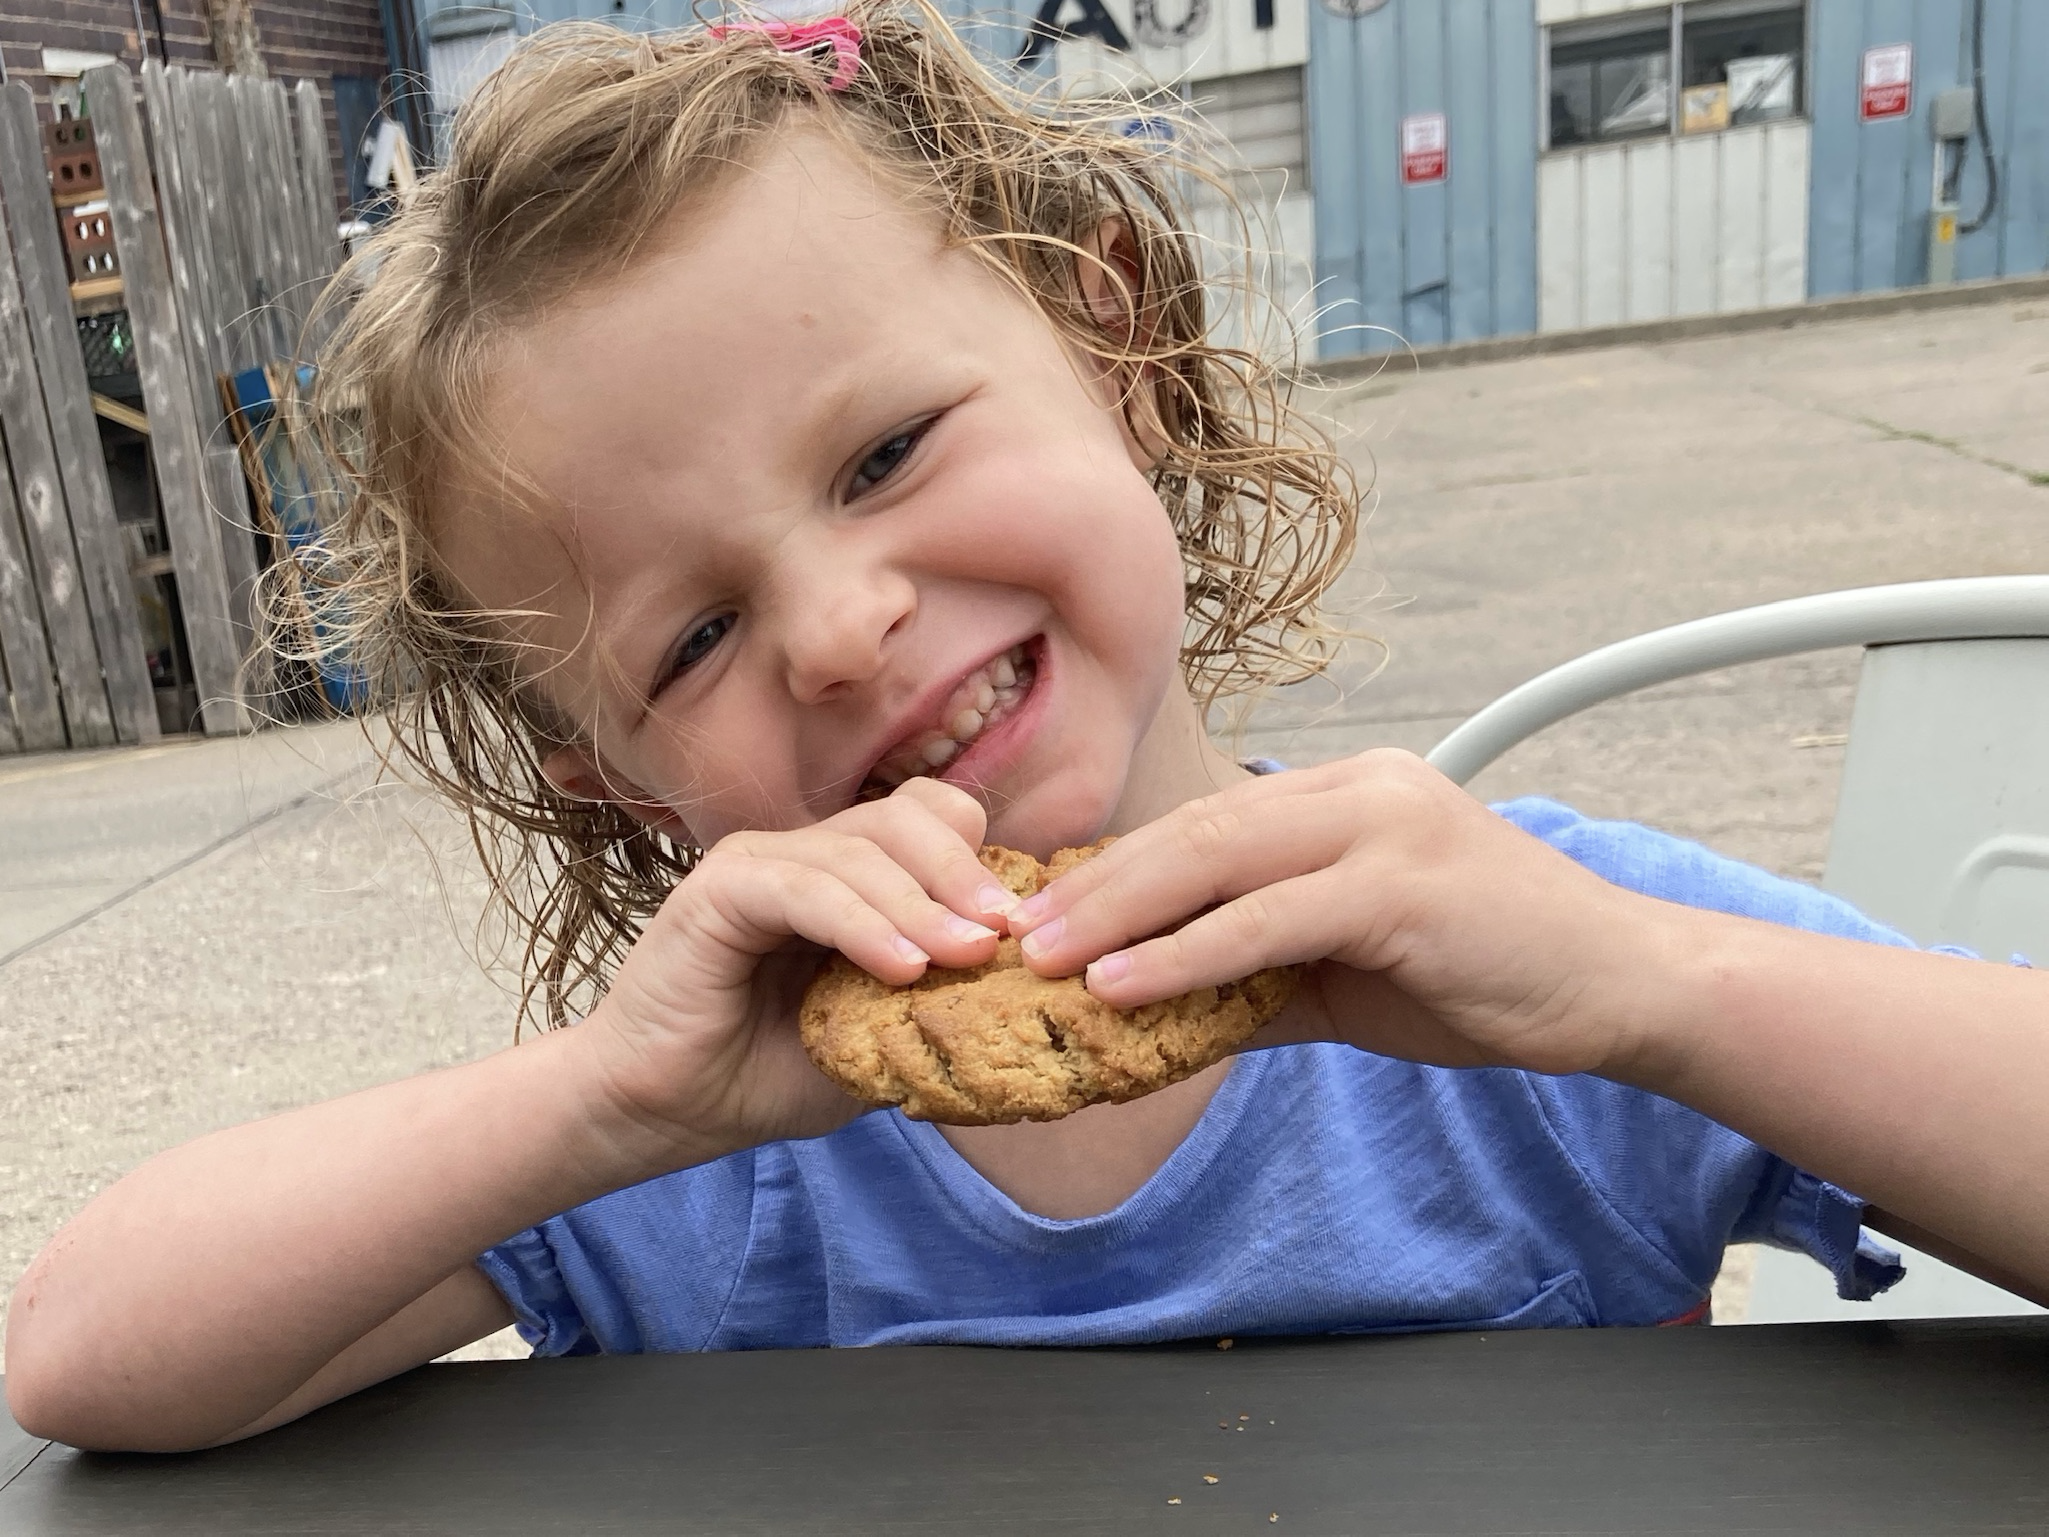
\includegraphics[width=5in]{img/lila.png}
		
		Lila (age 4)
	\end{center}

}


\frame{
	\frametitle{}
	
	\begin{center}
		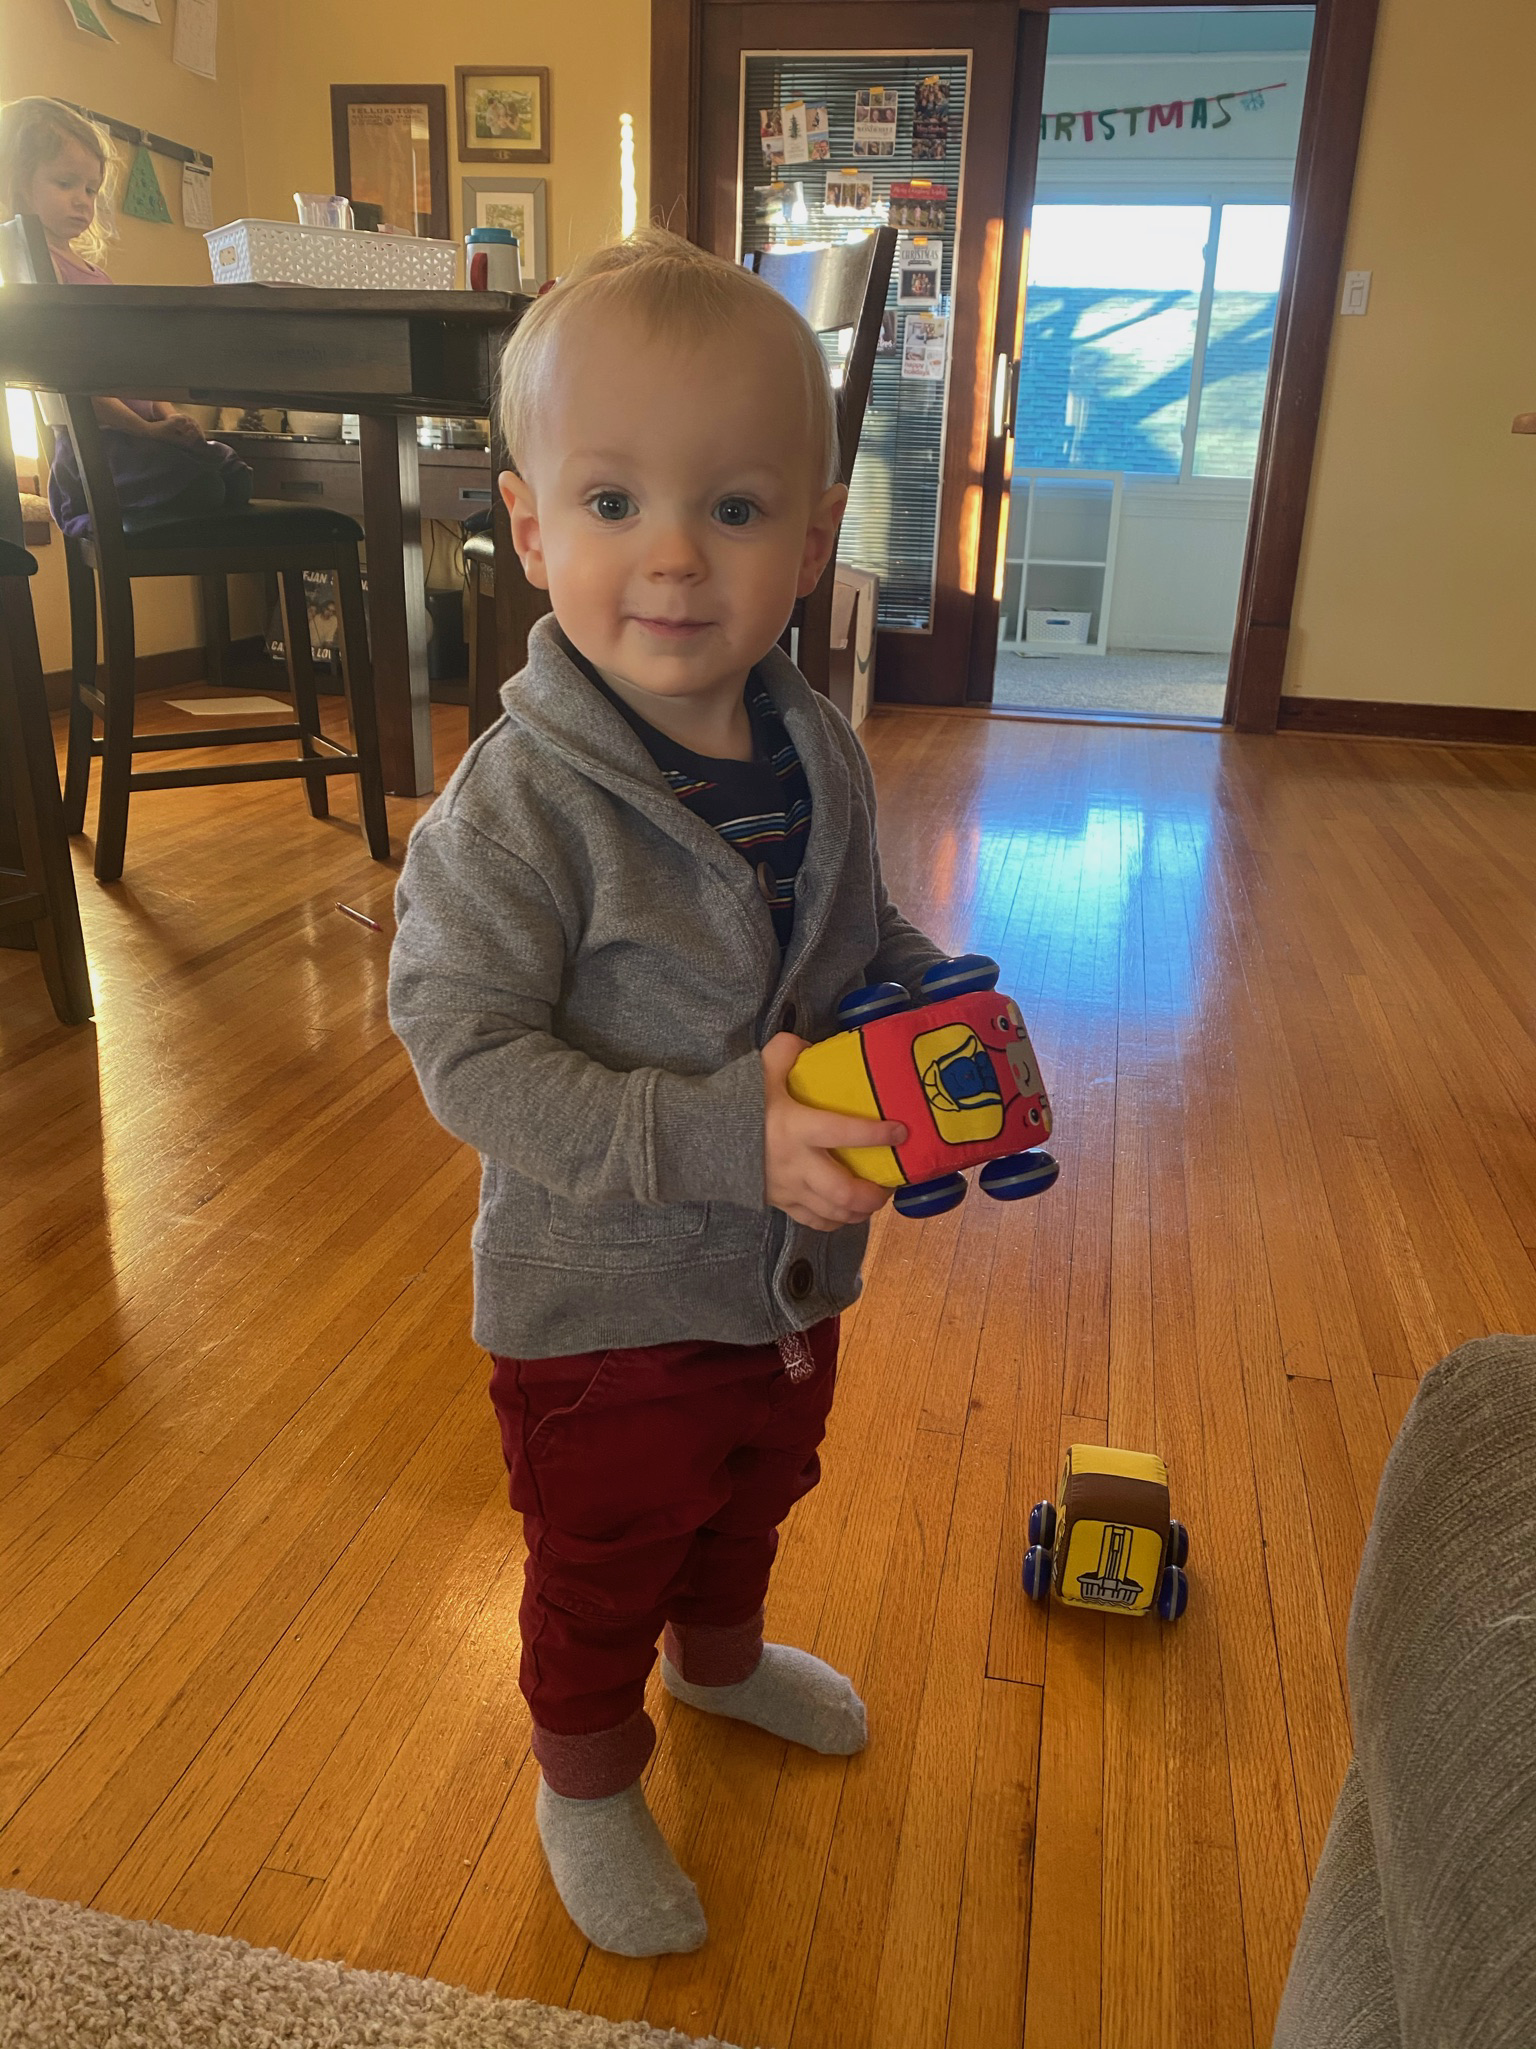
\includegraphics[width=2.5in]{img/sam.png}
		
		Sam (age 1)
	\end{center}

}

\frame{
	\frametitle{Agenda}
	
	Syllabus exploration
	
Expectations and Q\&A

The Big Idea of Calculus

Average Velocity

}

\section{Course Intro and Syllabus Exploration}



\frame{
	\frametitle{Activity: Scavenger Hunt}
	
	\begin{itemize}  
	\item Go to {\tt\alert{student.desmos.com}}
	
	\item Type in the class code:
	
	\begin{center}
		{\tt\large\alert{MYH RR5}}
	\end{center}
	
	\item Create an account to sign in (this will be required for the preview activities!)
	  
\end{itemize}

	

}

\section{Highlights}

\frame{
	\frametitle{ALEKS (I know you're sick of this)}
	
	\begin{itemize}
	\item Required score: 70 or better, by Monday
\item Not meeting this requirement could significantly disrupt your four-year plan
\end{itemize}

}

\frame{
	\frametitle{Required materials}
	
	\begin{itemize}
	\item Access to Canvas/Active Calculus/Edfinity
\item Calculus Bundle from Campus Store
\end{itemize}

}

\frame{
	\frametitle{Grading}
	
	\begin{itemize}
	\item Focus on mastery, not just getting things partly right
	\item Engagement Points: points for being a good citizen of the class
\item Mastery-based exams/quizzes
\item We’ll talk more about it as it becomes relevant
\end{itemize}

}

\frame{
	\frametitle{Student Hours Appointments}
	
	\begin{minipage}[c]{0.45\linewidth}
\begin{itemize}
	\item ``\emph{Student} Hours'' are \textbf{your} time!
\item Preferred method: make an appointment at\\ {\tt\small https://calendly.com/mkjanssen}
\item Appointments are \textbf{not} required
\item Drop in if my door is open!
\end{itemize}
\vspace{.25in}
\end{minipage}
\hspace{0.5cm}
\begin{minipage}[c]{0.45\linewidth}
\centering
\includegraphics[width=\textwidth]{img/calendly.png}
\end{minipage}

}

\section{Expectations}

\frame{
	\frametitle{Preparing for class}
	
	\begin{itemize}
	\item Look at each week’s Canvas homepage by Monday and note upcoming deadlines
\item Buy the calculus bundle and do the prep assignments

\item If you have a virtual accommodation, prepare to participate asynchronously after class.
\item Take care of yourself so you can actively engage in the class
\end{itemize}

}

\frame{
	\frametitle{In Class/Participating Remotely}
	
	\begin{itemize}
	\item Wear a mask that covers your mouth and nose for the duration of class
\item Try the activities and ask questions when you’re stuck. %—I’ll be wearing an AirPod for those watching live on Teams.
\item Talk to your neighbors and participate!
\item Use a visual cue to get attention—we can’t see if you’re about to say something!
\item Show grace toward one another (and me!) as we navigate an occasionally strange/awkward educational environment
\end{itemize}

}


\frame{
	\frametitle{After class}
	
	\begin{itemize}
	\item Make appointments with me! Or just drop by. I’m in SB 1612.
\item Complete the homework on time.
\item Upload your activities by 5pm on Fridays
\item Take the exams/quizzes seriously!
\end{itemize}

}

\frame{
	\frametitle{Collaboration}
	
	\begin{itemize}
	\item Collaboration is encouraged! 
\item All work that you turn in must be your own.
\item If you discuss a problem with someone at all, you should say so.
\end{itemize}

}

\section{Questions?}


\section{Thinking about velocity}

\frame{
	\frametitle{Preview Activity 1.1.1}
	
	\begin{itemize}
	\item 	Work with those nearby 
	\item Goal: put forth a good-faith effort on each problem
	\item Remember that your work will be scanned and uploaded for good-faith effort by the end of the week, so take good clean notes in your workbooks
\end{itemize}

}





\frame{
	\begin{center}
		\includegraphics[width=3in]{img/pa111.png}
	\end{center}

}


\frame{
	\frametitle{Position v.~Velocity}
	
	\begin{itemize}
	\item When position is happening along a line, it can be described by a single variable function $s(t)$\pause
	\item Units: $t$ is time, $s(t)$ is distance\pause
	\item Average velocity from $t = a$ to $t= b$:
	
	\[
		AV_{[a,b]} = \frac{s(b) - s(a)}{b-a}
	\]
\end{itemize}

}

\frame{
	\frametitle{Activity 1.1.2}
	

}

\frame{
	\frametitle{The Infinity Principle}
	
	\begin{quote}
	To shed light on any continuous shape, object, motion, process, or phenomenon—no matter how wild and complicated it may appear—reimagine it as an infinite series of simpler parts, analyze those, and then add the results back together to make sense of the original whole.
	\end{quote}
	
	--Steven Strogatz, \textit{Infinite Powers}

}

\frame{
	\frametitle{``Instantaneous Velocity'' is Nonsense...}
	
	\begin{itemize}
	\item \alert{Question:} What can we measure in an instant (e.g., in a photograph)?\pause
	\item \textbf{However:} velocity is a \emph{rate of change}--at any given \emph{instant}, I am not moving!\pause
	\item The Infinity Principle gives us a way of approximating something like ``instantaneous velocity''
\end{itemize}

}


\frame{
	\frametitle{...but we can define it anyway}
	
	\begin{itemize}
	\item The idea: to approximate instantaneous velocity at $t = a$, compute the average velocity over the interval $[a,a+h]$, where $h$ is some arbitrarily (infinitesimally?) small number that is allowed to vary \rem{$h < 0$?}\pause
	\item That is:
	\[
		IV_{t=a} \approx AV_{[a,a+h]} = \frac{s(a+h) - s(a)}{a+h -a} = \frac{s(a+h) - s(a)}{h}
	\]
\end{itemize}

}

\frame{
	\frametitle{Example}
	
	In a time of $t$ seconds, a particle moves a distance of $s(t) = 4t^2 + 3$ meters from its starting point. Find an expression for the average velocity on $[1,1+h]$, and use it to estimate the instantaneous velocity of the particle at $t=1$. 
	
	\vspace{2in}

}

\frame{
	\frametitle{Activity 1.1.4}

}

%\section{Bonus}


\frame{
	\frametitle{For Next Time}
	
	\begin{itemize}
	\item Pass the ALEKS
\item Buy the calculus bundle from the campus store (\~\$60)
\item Complete the Edfinity demo assignment
\item Do the Section 1.2 Prep assignment by 8am Monday
\item Talk to me if you have any questions!
\end{itemize}

}


\end{document}